\documentclass{article}
\usepackage[utf8]{inputenc}
\usepackage{amsmath, amsthm, amssymb, amsfonts}
\usepackage{matlab-prettifier}
\usepackage[margin=1in]{geometry}
\usepackage{graphicx}



\title{CompEcon - Problem Set 1}
\author{Yuna Aulia and Ruggero Jappelli}
\date{January 2019}

\begin{document}

\maketitle

\section*{Problem 1}
\subsection*{1}
\noindent
The market equilibrium is characterized by the equality between Supply and Demand. Therefore:
\begin{equation}
\nonumber
\begin{aligned}
& S = D\\
& a - bq = c + dq\\
& 0 = c + dq - a + bq\\
& 0 = bq + dq - (a - c)
\end{aligned}
\end{equation}

\subsection*{2}
From (1):
\begin{equation}
\nonumber
\begin{aligned}
& q = \frac{a - c}{b + d}
\end{aligned}
\end{equation}

Plug (2) into the demand function:
\begin{equation}
\nonumber
\begin{aligned}
& p = a - bq\\
& p = a - b \frac{a - c}{b + d}\\
& p = a - \frac{ab - bc}{b + d}
\end{aligned}
\end{equation}

Plug (2) into the supply function:
\begin{equation}
\nonumber
\begin{aligned}
& p = c + dq\\
& p = c + d \frac{a - c}{b + d}\\
& p = c + \frac{ad - cd}{b + d}
\end{aligned}
\end{equation}

\subsection*{3}
$$
\underbrace{ \begin{pmatrix}
1&b\\
1&-d\\
\end{pmatrix}}_\text{A}
\underbrace{\begin{pmatrix}
p\\
q\\
\end{pmatrix}}_\text{x}
=
\underbrace{\begin{pmatrix}
a\\
c\\
\end{pmatrix}}_\text{y}
$$

Breaking matrix A into LU:

$$
\begin{pmatrix}
1&0\\
0&1\\
\end{pmatrix}
\vline
\begin{pmatrix}
1&b\\
1&-d\\
\end{pmatrix}
\xrightarrow{r2 - r1}
\underbrace{\begin{pmatrix}
1&0\\
-1&1\\
\end{pmatrix}}_\text{L}
\vline
\underbrace{\begin{pmatrix}
1&b\\
0&-d - b\\
\end{pmatrix}}_\text{U}
$$

Therefore we can describe this as LUx = y. Let us assume Ux = z, therefore Lz = y.
$$
\underbrace{\begin{pmatrix}
1&0\\
-1&1\\
\end{pmatrix}}_\text{L}
\underbrace{\begin{pmatrix}
z_1\\
z_2\\
\end{pmatrix}}_\text{z}
=
\underbrace{\begin{pmatrix}
a\\
c\\
\end{pmatrix}}_\text{y}
$$

This will create a new system of linear equation:

\begin{equation}
\nonumber
\begin{aligned}
z_1 = a
\end{aligned}
\end{equation}

\begin{equation}
\nonumber
\begin{aligned}
-z_1 + z_2 = c \rightarrow z_2 = c - a
\end{aligned}
\end{equation}

And from Ux = z
$$
\underbrace{\begin{pmatrix}
1&b\\
0&-d - b\\
\end{pmatrix}}_\text{U}
\underbrace{\begin{pmatrix}
p\\
q\\
\end{pmatrix}}_\text{x}
=
\underbrace{\begin{pmatrix}
a\\
c - a\\
\end{pmatrix}}_\text{z}
$$

Solving for x: 
\begin{equation}
\nonumber
\begin{aligned}
(-d - b)q = c - a \rightarrow q = \frac{a - c}{b + d} 
\end{aligned}
\end{equation}

\begin{equation}
\nonumber
\begin{aligned}
p + bq = a\\
p = a - bq\\
p = a - b \frac{a - c}{b + d}
\end{aligned}
\end{equation}

\subsection*{4}
\begin{equation}
\nonumber
\begin{aligned}
q = \frac{a - c}{b + d} = \frac{3 - 1}{0.5 + 1}= \frac{4}{3}
\end{aligned}
\end{equation}

\begin{equation}
\nonumber
\begin{aligned}
p = a - b \frac{a - c}{b + d} = 3 - \frac{1}{2}\bigg(\frac{3 - 1}{0.5 + 1}\bigg) = \frac{7}{3}
\end{aligned}
\end{equation}

\subsection*{5}

\textbf{Matlab code for Gauss - Seidel Method}
\lstinputlisting[style = Matlab-editor]{Exercise1.m}
\subsection*{6}

\textbf{Matlab code for Iteration using Successive Over Relaxation}
\lstinputlisting[style = Matlab-editor]{Exercise1.m}

\section*{Problem 2}
\textbf{Matlab code for Output Gap}
\lstinputlisting[style = Matlab-editor]{Exercise2.m}

\subsection*{5}
\begin{figure}[c]
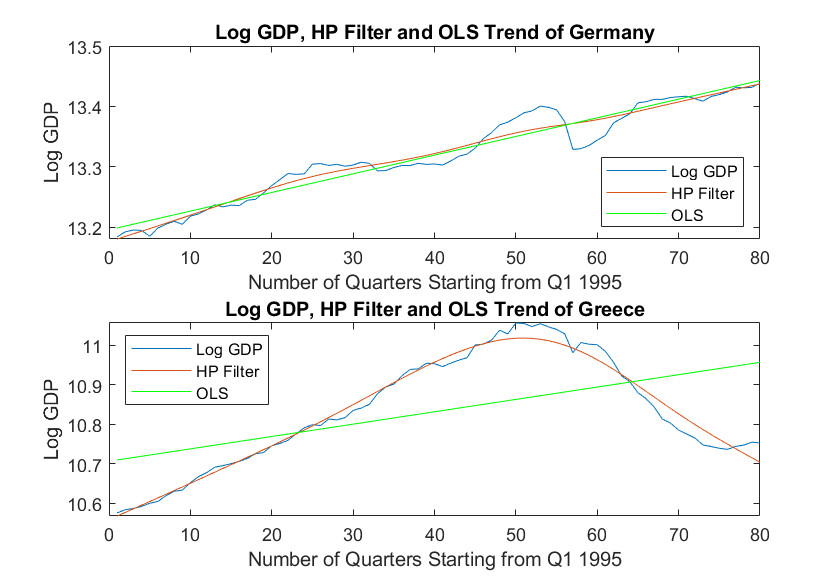
\includegraphics[height=12cm, width=\textwidth]{fig2_1}
\caption{Log GDP Versus Trend}
\end{figure}
\begin{figure}[c]
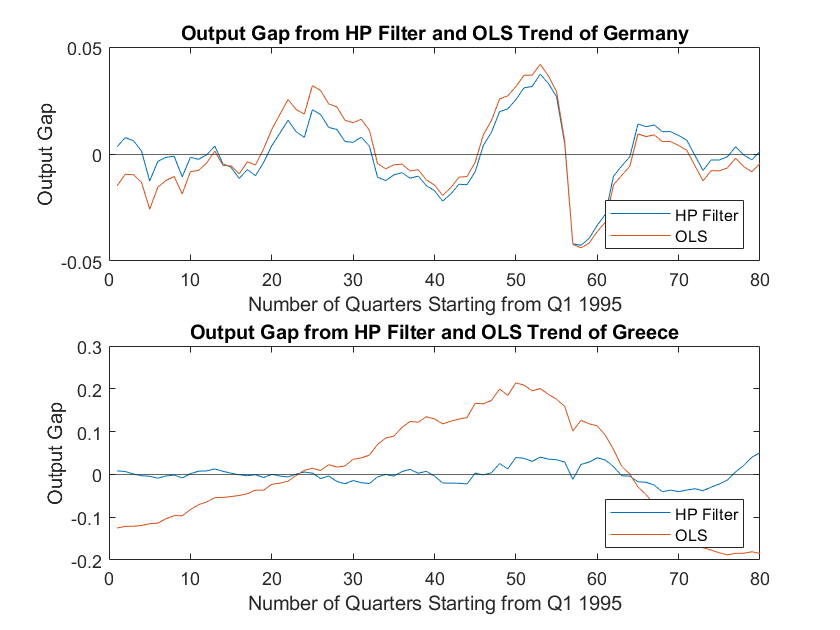
\includegraphics[height=12cm, width=\textwidth]{fig2_2}
\caption{Output Gap}
\end{figure}

\pagebreak


\pagebreak

\section*{Problem 3}
\subsection*{1}
\textbf{Matlab Code for Bisection Algorithm}
\lstinputlisting[style = Matlab-editor]{Exercise3.m}
\\subsection*{2}
We use the bisection method to compute the zeroes of the following functions: \\
The function $$f(x) = x^3 + 4 - 1/x$$ has a root $x = 0.249038$\\

The function $$f(x) = -exp(-x) + exp(-x^2) $$ has a root $x = 0$ and a root at $51$, obtained varying the starting points.

\subsection*{3}
$$b \times q + d \times q^\phi - (a - c) = 0 $$
Assume $$ a = 3, b = 0.5, c = d = 1, \psi = 0.5$$
We then have $$ \dfrac{q}{2} + \sqrt{q} -2 = 0 $$
  analytical solution:   \\
$$ q = (2 - \dfrac{q}{2})^2$$
$$ q = 4 +\dfrac{q^2}{4} - 2q  $$
$$ 0 = \dfrac{q^2}{4} - 3q + 4 $$
$$ q^2 - 12q + 16 = 0$$
$$ q = \dfrac{12 \pm \sqrt{12^2 - 64}}{2}$$
The positive solution is 1.527864045. \\
  The solution computed with the bisection method is 1.52786 \\
  Similarly, with the matlab built-in function fzero the solution is: 1.527864045000420 \\
  
  
  \section*{Problem 4 - A Contribution to the Empirics of Economic Growth}
   \begin{center}
      \textbf{Matlab Code for Exercises 4.1}
  \end{center}
  We load the data with import data as a table, excluding rows with unimportable cells. After cheching with the matlab function isnan, we have 104 countries in our dataset.\\
  \begin{center}
      \textbf{Matlab Code for Exercises 4.2-4.3}
  \end{center}
\lstinputlisting[style = Matlab-editor]{Exercise4.m}

  \\
  \\\subsection*{4}
  \begin{table}[htbp]\centering \caption{Summary statistics \label{sumstat}}
\begin{tabular}{l c c c}\hline\hline
\\ 
  \multicolumn{3}{c}{\textit{Dependent variable: log difference GDP per working-age person 1960-1985 }} \\ 
\\[-1.8ex]  
            &\multicolumn{1}{c}{(Non Oil)}&\multicolumn{1}{c}{(Intermediate)}&\multicolumn{1}{c}{(OECD)}\\
            &\multicolumn{1}{c}{OLS}&\multicolumn{1}{c}{OLS}&\multicolumn{1}{c}{OLS}\\
\hline\hline\\[-1.8ex] 
CONSTANT  & 1.112436013441833 & 1.655664821192208 & 2.611627292608531\\
log(gdp1960) & -0.296562179734063 & -0.373493872465916 & -0.399271205189533\\
log(I/y)  & 0.521228337626152 & 0.536026177101351 &  0.353093631576787\\
log(popgrowth + g + $\delta$) & -0.181085002271978 & -0.187462038101107 & -0.215690701932586\\
log(school)  & 0.233556041609175 & 0.273303053483721 & 0.235819465739553\\
\hline\hline\\[-1.8ex] 
\(N\)       &        98         &       75          &        22\\
\hline\end{tabular}
\end{table}
The coefficients in the table mirror very closely the ones in Table V in A Contribution to
the Empirics of Economic Growth \footnote{Mankiw, Romer, and Weil (1992), The Quarterly Journal of Economics, Vol. 107(2), pp. 407-437}, with the exception of log(popgrowth + g + $\delta$), since it is different by construction, and consequently the CONSTANT terms. All the other coefficient estimates are consistent with the results in Mankiw, Romer, and Weil (1992).
\end{document}
